
% !TeX root = ../treemap-taxonomy-ivapp2020.tex

%
{%
	\footnotesize
	\centering%
	%\newlength{\definitionswidth}%
	%\newlength{\definitionsheight}%
	%\newlength{\definitionsoffset}%
	%\newlength{\definitionsimagesize}%
	%\newlength{\definitionsdescriptionsize}%
	\setlength{\definitionswidth}{\textwidth}%
	\setlength{\definitionsheight}{145pt}%
	\setlength{\definitionsoffset}{6pt}%
	\setlength{\definitionsimagesize}{0.25\definitionswidth - 2\definitionsoffset}%
	\setlength{\definitionsdescriptionsize}{0.25\definitionswidth - 0.5\definitionsoffset}%
	\begin{tikzpicture}[]
	% Images
	\node[inner sep=0,outer sep=0] (space-filling) at (-1.5\definitionsimagesize - 3\definitionsoffset, 0.5\definitionsheight) {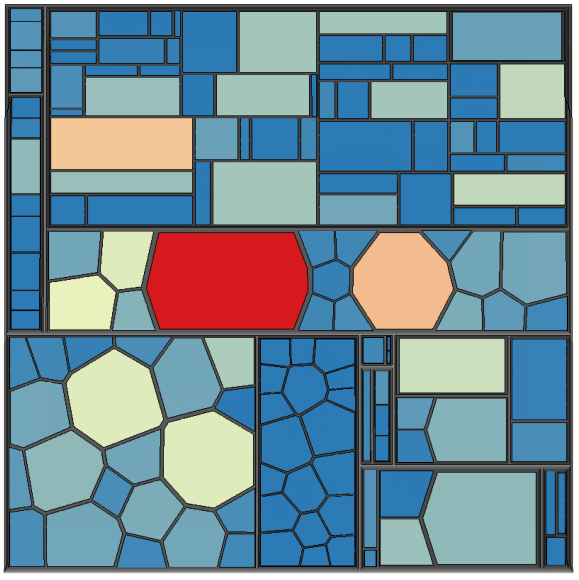
\includegraphics[width=\definitionsimagesize]{figures/mixed-treemap-layouting.png}};
	\node[inner sep=0,outer sep=0] (containment) at (-0.5\definitionsimagesize + -1\definitionsoffset, 0.5\definitionsheight) {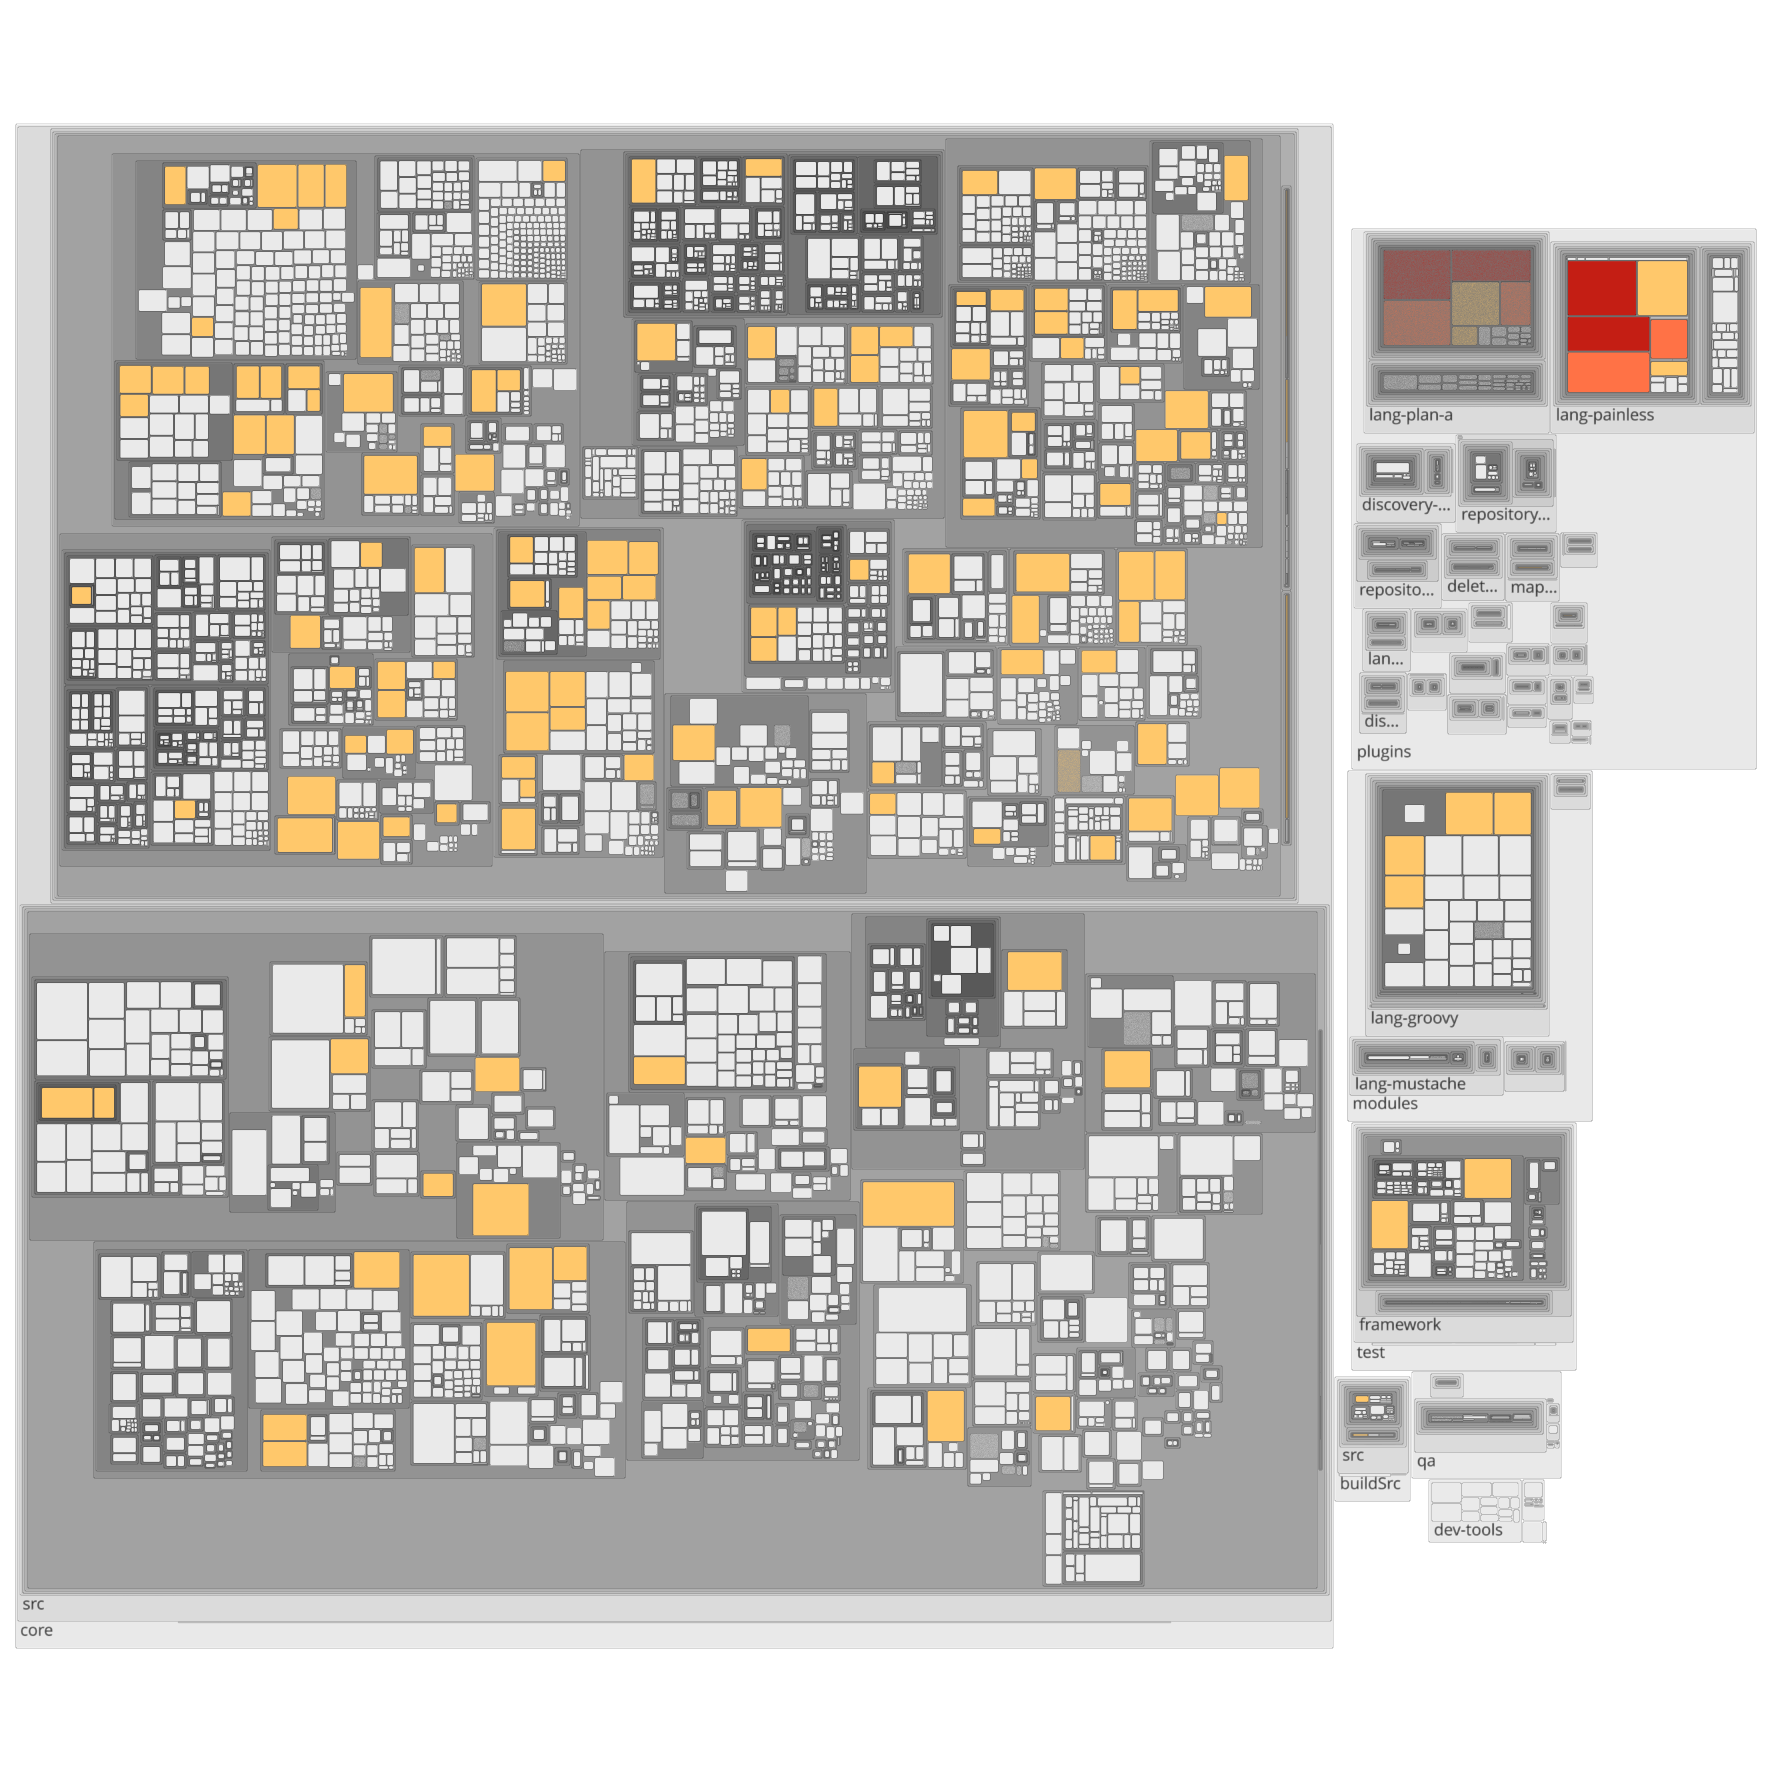
\includegraphics[width=\definitionsimagesize]{figures/evocells.png}};
	\node[inner sep=0,outer sep=0] (implicit-edge) at (0.5\definitionsimagesize + 1\definitionsoffset, 0.5\definitionsheight) {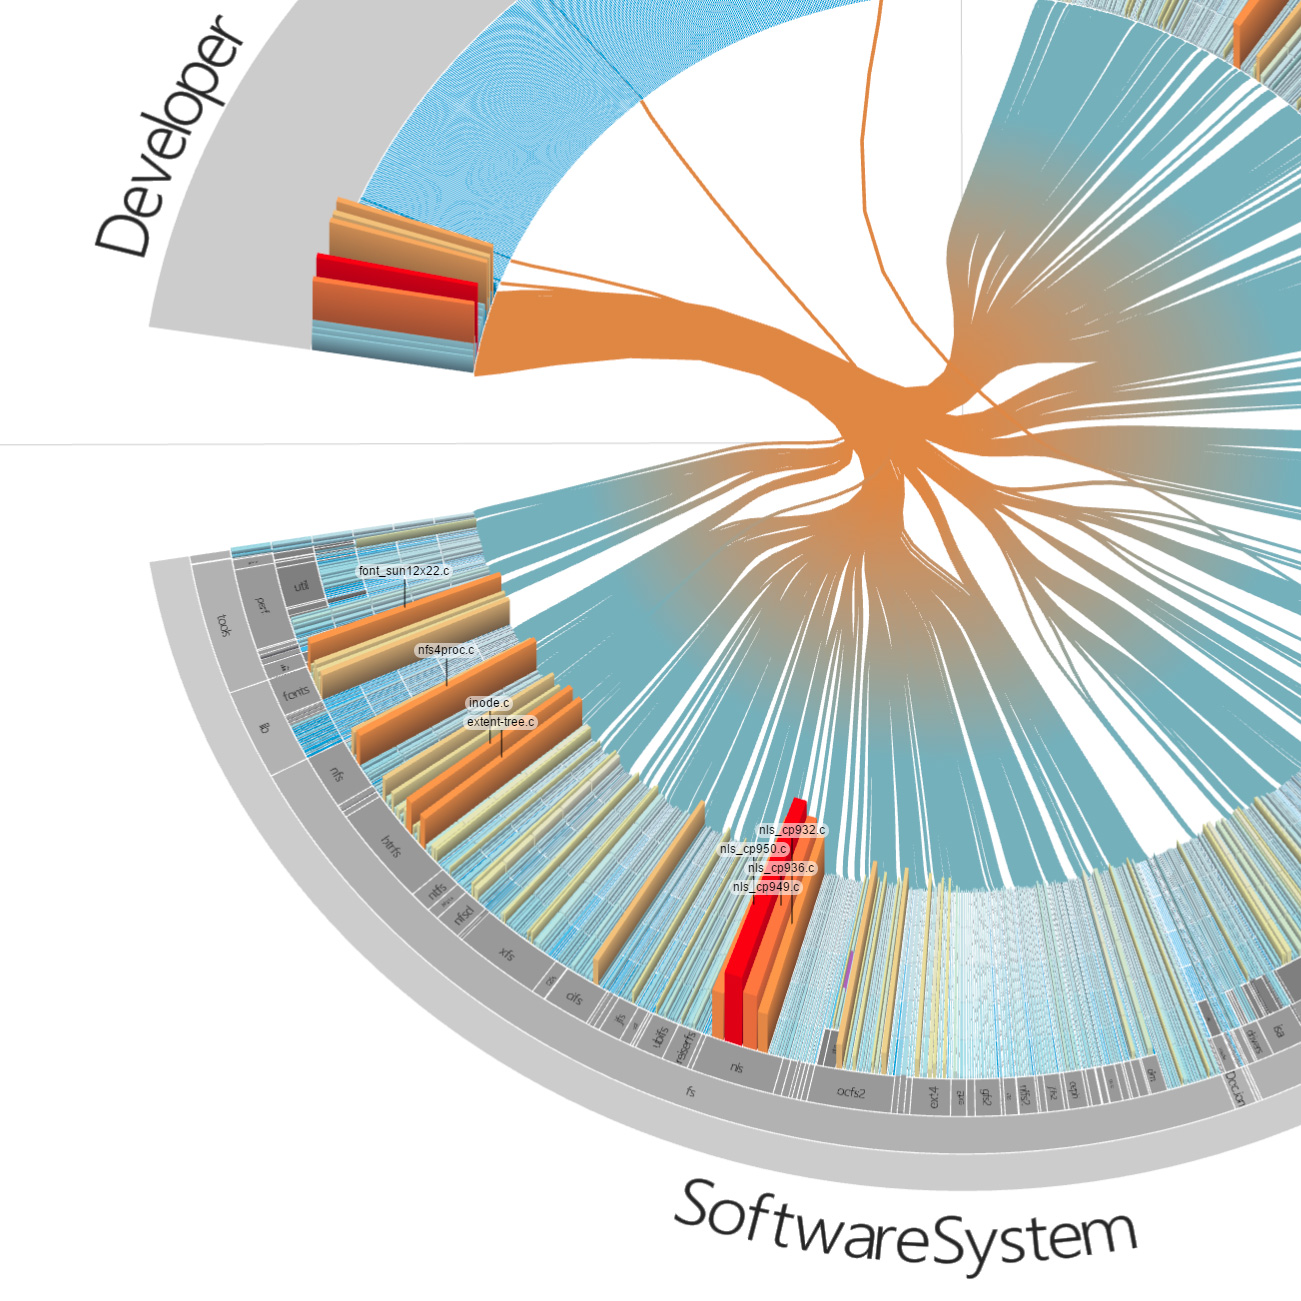
\includegraphics[width=\definitionsimagesize]{images/circular-bundle-view-bp.jpg}};
	\node[inner sep=0,outer sep=0] (mapped-tree) at (1.5\definitionsimagesize + 3\definitionsoffset, 0.5\definitionsheight) {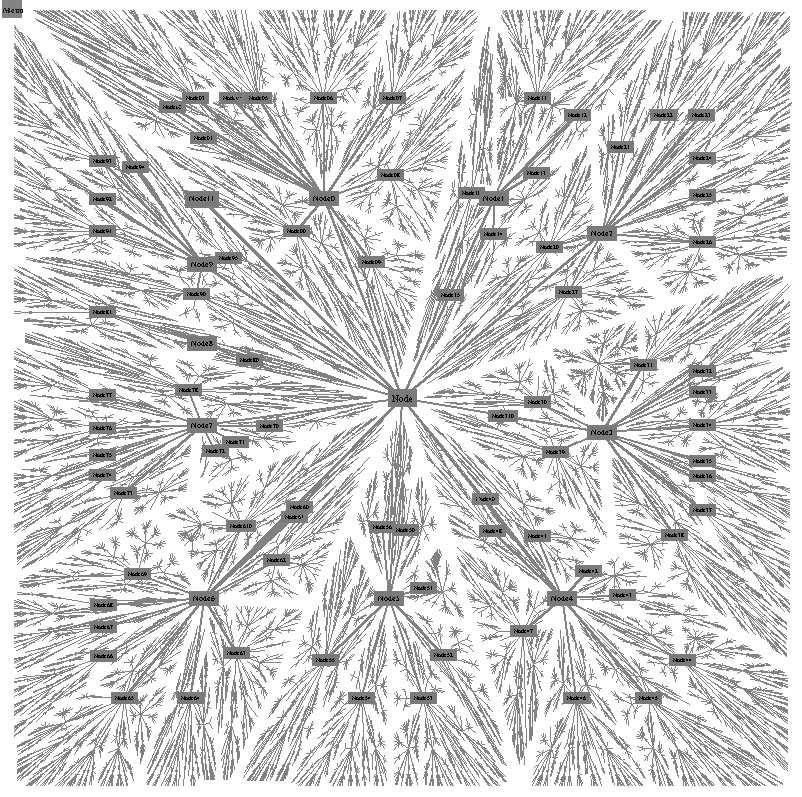
\includegraphics[width=\definitionsimagesize]{figures/spaceoptimizedtree.png}};
	\end{tikzpicture}%
}%
%
